\documentclass[a4paper,12pt, titlepage]{article}
\usepackage[finnish]{babel} %suomenkielinen tavutus
\usepackage[T1]{fontenc} %skanditavutus
\usepackage[utf8]{inputenc}        	% skandit utf-8 koodauksella
%\usepackage[ansinew]{inputenc}        	% skandit utf-8 koodauksella, kokeile tata, jos utf-8 ylla ei toimi.

\usepackage{graphicx}
\usepackage{hyperref}
\usepackage{tabularx}

\linespread{1.24} %rivivali 1.5
\sloppy % Vahentaa tavutuksen tarvetta, "leventamalla" rivin keskella olevia valilyönteja.


\title{Helpperin testaus}
\author{ Maiju Airosmaa \\ Kalle Hiljanen \\
Outi Jussila \\ Eetu Mattila \\ Johanna Vehniäinen \\[1cm] Ohjelmiston testausdokumentaatio \\ Helsingin yliopisto}
\date{Heinäkuu 2016}

\begin{document}

\maketitle

\newpage
\tableofcontents
\newpage

\section{Miten testaus on toteutettu}

Käytimme testauksessa Rspec:iä. Luokille on kirjoitettu yksikkötestejä ja toiminnallisuutta olemme testanneet selaintason käyttöliittymätesteillä Capybaralla. Testeissä käytettiin laajasti FactoryGirlillä tehtyjä fixtureja. Selaintason testit on tehty lähinnä mustalaatikko-toteutuksena, jossa sovelluksen backendin tuntemusta ei tarvita.

Testejä ajoimme jatkuvasti lokaalisti uusien ominaisuuksien lisäämisen jälkeen, koska pienetkin lisäykset ja muutokset vaikuttivat testeihin. Tarvittaessa korjasimme joko koodia tai testejä. Testit ajettiin myös Travis-CI-palvelimella aina, kun pushasimme muutoksia GitHub-repositorioon.

\section{Testikattavuus}

Tavoitteenamme oli alusta lähtien pitää testien rivikattavuus korkealla, joten testejä on kirjoitettu sitä mukaa, kun uusia ominaisuuksia lisättiin. Alussa testejä kirjoitettiin huomattavasti laajemmin, mutta huomasimme pian, että koodin muuttuessa jouduimme jatkuvasti korjaamaan jo olemassa olevia testejä. Testejä tuli myös kirjoitettua päällekkäin eli yksikkö ja käyttöliittymätestit testasivat samoja asioita. Näiden huomioiden jälkeen vähensimme testien kirjoittamista pitäen rivikattavuuden kuitenkin korkealla. Myös sprinttien lyhyt kesto vaikutti testaamisen laajuuteen, koska aika tuntui jatkuvasti loppuvan kesken. Definition of Donin mukaan testikattavuuden tavoitteemme oli 90\%. Projektin puolessa välissä testikattavuus laahasi 70\%:n tuntumassa, koska lisäsimme Scaffoldilla luokan Category, mutta tämän luokan kontrolleria ei testattu, koska sillä ei ollut käyttöä sovelluksessa. Kategoriat luotiin seedillä ja niiden poistaminen täytyi olla mahdotonta. Jätimme kuitenkin varsinaisen sovelluksen ulkopuoliseksi ominaisuudeksi mahdollisuuden muokata kategorioita muutenkin kuin konsolin kautta. Myöhemmässä vaiheessa ignoroimme kyseessä olevan kontrollerin testikattavuuden ulkopuolelle .simplecov-tiedostossa. Samassa tiedostossa ignoressa ovat myös admin- ja info-kontrollerit. Admin- ominaisutta emme ehtineet toteuttamaan ollenkaan ja info-kontrollerin metodeilla ei ole mitään sisältöä. Näiden tiedostojen ignoroimisen jälkeen testikattavuus pysyi jatkuvasti tavoitteessa tai hyvin lähellä sitä. Lopullinen testikattavuus oli noin 93\%:a.
Testikattavuuden tarkasteluun käytimme lokaalisti Simplecov:ia. Jos testit menivät palvelintasolla läpi Travisista, niin lähetettiin kattavuusraportti Coverallsiin.

\section{Liitteet}

Travis-CI:
\url{https://travis-ci.org/xjoxjox/helpperi}
\newline
Coveralls:
\url{https://coveralls.io/github/xjoxjox/helpperi}
\newline
\newline
Simplecovin kattavuusraportti:
\newline
\newline
\noindent\makebox[\textwidth]{%
\begin{tabularx}{1.5\textwidth}{XX}
  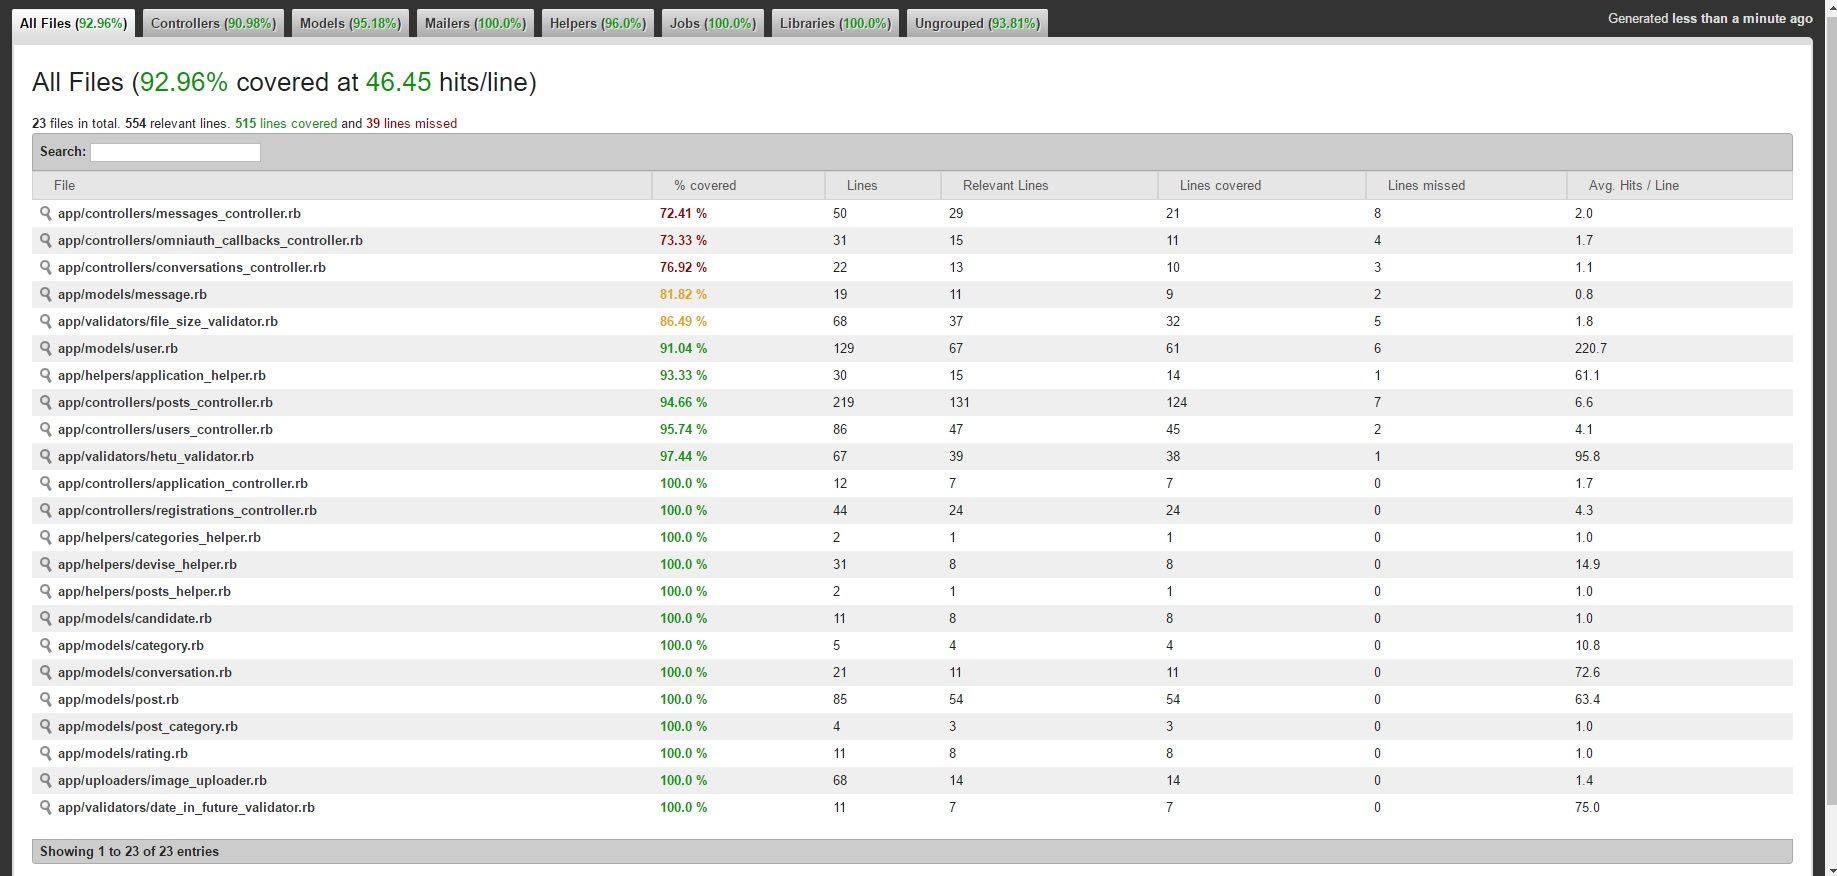
\includegraphics[width=200mm]{kattavuus}
\end{tabularx}}




\end{document} 